\documentclass[../report.tex]{subfiles}

\begin{document}

\chapquote{The beauty of a move lies not in its appearance but in the thought behind it.}{Aron Nimzowitsch}
\chapter{Adapting to unseen chess sets}
\label{chap:adapting}

Chess sets may vary significantly in appearance. 
As a result, \glspl{cnn} trained on one type of chess set might perform poorly in the inference stage when supplied with images of another chess set. 
This is because we violate the assumption that the training and testing data are drawn from the same distribution.
In light of the theory introduced in \cref{sec:background_transfer_learning}, the natural response is to employ transfer learning in order to fine-tune the \glspl{cnn} to this new data distribution.
Due to the inherent similarities in the data distribution (the fact that they are chess sets and that the source and target tasks are the same), it stands to reason that we could employ a form of \emph{one-shot} transfer learning; 
that is, using only a small amount of data in order to adapt the \glspl{cnn} to the new distribution.
Using the least amount of data necessary makes the system considerably more convenient for the user.

A significant advantage of the chess recognition system as it is developed in \cref{chap:chess_recognition} is the fact that we employ conventional computer vision techniques such as edge and line detection in order to localise the board.
This means that we are able to find the location of practically \emph{any} type of chess board with a high accuracy, not just the board used to generate the training data.
On the other hand, had we employed a board localisation technique based on deep neural networks (for instance a semantic segmentation model), the system would suffer the same type of issues as the \glspl{cnn} mentioned above when required to adapt to new chess sets.
The fact that we can reliably find the corner points of any chess board but may not be able to correctly identify the configuration of pieces on the board gives rise to a system where we could employ transfer learning to obtain better predictions with only minimal extra effort on the part of the user:
if the user wants to employ our system to infer a position on their own chess board, they just need to take a picture of the starting position (\cref{fig:chess_start_position}) from both players' perspectives.
\begin{figure}[h]
    \centering
    \newgame
    \showboard
    \caption[The starting position on the board.]{The starting position on the board. It is the same at the beginning of each game, thus a photo captured in this position is well-suited for transfer learning as the user does not need to manually label the position.}
    \label{fig:chess_start_position}
\end{figure}
The angle of the camera to the chessboard should be in the same interval as used in the data synthesis process depicted in \cref{fig:camera_angle}, i.e.\ between 45° and 60°.
This chapter will demonstrate how to effectively fine-tune the occupancy and piece classification \glspl{cnn} based on only two input images.

\section{Dataset}
First, we require a dataset in order to evaluate the effectiveness of our approach.
The training set, consisting of the two images obtained in the aforementioned manner is depicted in \cref{fig:transfer_learning_train_data}.
\begin{figure}
    \centering
    \begin{subfigure}[b]{0.47\textwidth}
        \centering
        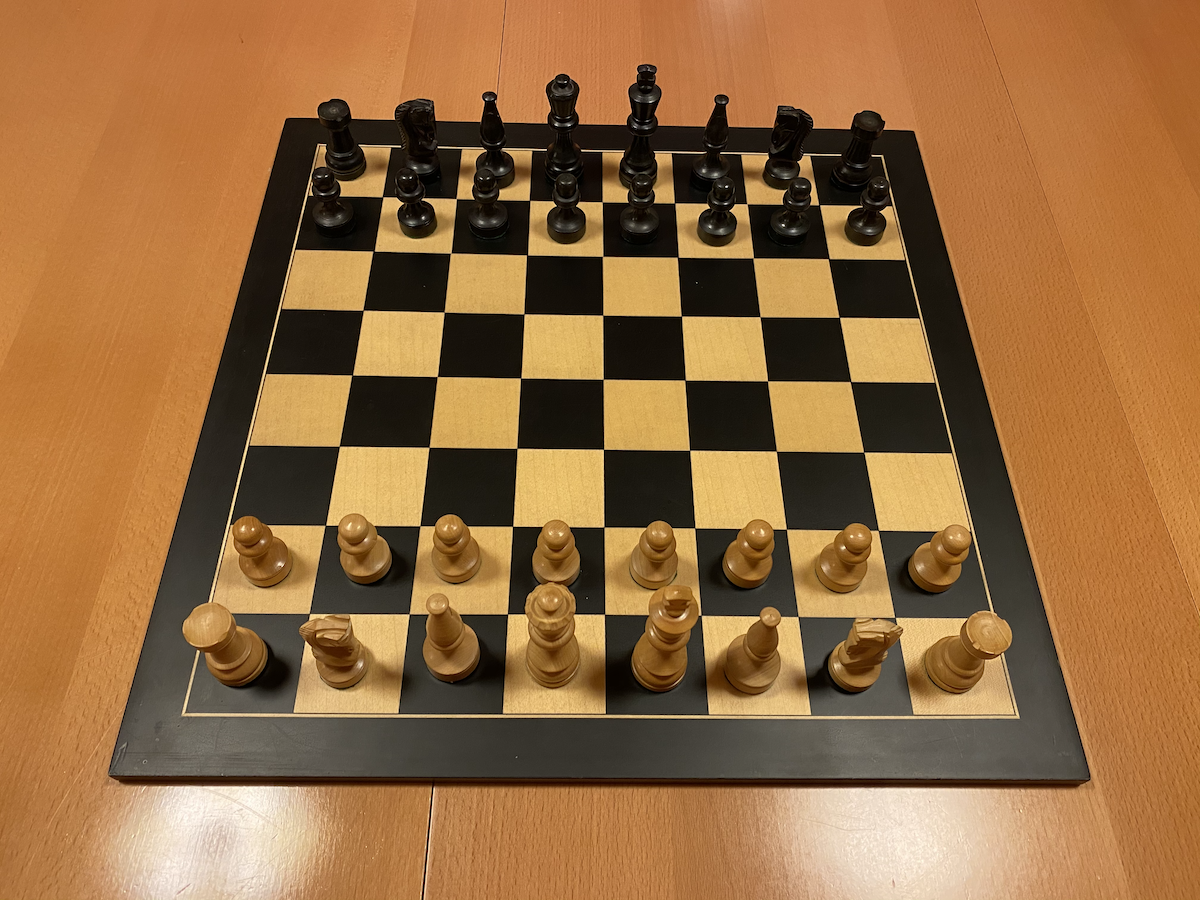
\includegraphics[width=\textwidth]{transfer_learning_white}
        \caption{white player's perspective}
    \end{subfigure}
    \hfill
    \begin{subfigure}[b]{0.47\textwidth}
        \centering
        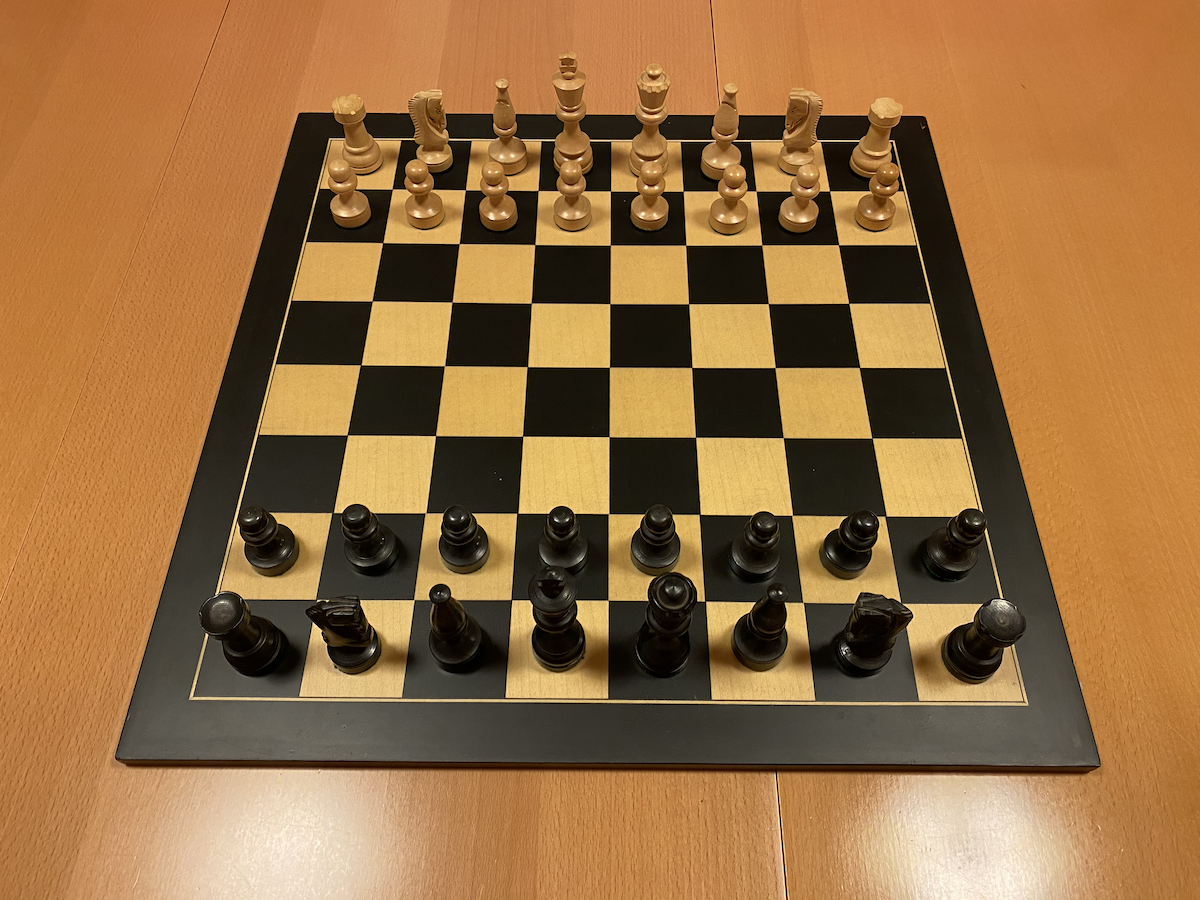
\includegraphics[width=\textwidth]{transfer_learning_black}
        \caption{black player's perspective}
    \end{subfigure}
    \caption{The training dataset used for the transfer learning approach, consisting of only two samples.}
    \label{fig:transfer_learning_train_data}
\end{figure}
For this task, we do not employ a validation dataset because the availability of labelled data is limited (it would be unreasonable to ask the user for more photos and then even requiring them to manually annotate the positions).
The test dataset consists of 27 images which were obtained by playing a game of chess and taking a photo of the board after each move.
Each photo is taken from the current player's perspective, so the images alternate between White's and Black's perspectives.
All samples are associated with a manually labelled \gls{fen} string describing the position.

At this point, it is a good idea to establish a baseline for the quality of predictions the chess recognition pipeline achieves without fine-tuning the \glspl{cnn} on the test set.
These results are summarised in \cref{tbl:transfer_learning_results_without_finetuning}.
\begin{table}
    \centering
    \begin{tabular}{lrr}
        \toprule
        metric & training set & test set \\
        \midrule
        mean number of incorrect squares per board           & 9.50     & 9.33 \\
        percentage of boards predicted with no mistakes      & 0.00\%   & 0.00\%   \\
        percentage of boards predicted with $\leq 1$ mistake & 0.00\%   & 0.00\%   \\
        per-board corner detection accuracy                  & 100.00\% & 100.00\% \\
        per-square occupancy classification accuracy         & 100.00\% & 99.88\% \\
        per-square piece classification accuracy             & 85.16\%  & 85.52\% \\
        \bottomrule
    \end{tabular}
    \caption[Performance of the chess recognition pipeline from \cref{chap:chess_recognition} on the transfer learning dataset without fine-tuning.]{Performance of the chess recognition pipeline from \cref{chap:chess_recognition} on the transfer learning dataset without fine-tuning. In this case, the training set is not used for training because the model is not fine-tuned.}
    \label{tbl:transfer_learning_results_without_finetuning}
\end{table}
This regime is unable to completely identify any of the positions; on average, it misclassifies 9.33 out of 64 squares per board.
The accuracy of the corner detection algorithm is 100\%, meaning that it can generalise nicely to new chess sets as hypothesised at the beginning of this chapter.
While the occupancy classification \gls{cnn} is able to adapt quite well to this new dataset as well (achieving an accuracy of 99.88\% on the test set), the underlying reason for the poor performance stems from the piece classifier that achieves only around 85\% accuracy.

\section{Training}
The ability to fine-tune the models to this new dataset is mainly constrained by the limited availability of data.
Since we only have two input images, the occupancy classifier must be fine-tuned using only 128 samples (each board has 64 squares).
Moreover, the piece classifier has only 64 training samples because there are 32 pieces on the board at the starting position.
While the \gls{cnn} for occupancy detection is a binary classifier, the piece classifier must undertake the more challenging task of distinguishing between a dozen different piece types.
Furthermore, the data is not balanced between the classes: for example, there are 16 training samples for black pawns, but only two for the black king, and some pieces are more difficult to detect than others (pawns usually look the same from all directions whereas knights do not).
Given this premise, it is clear that we should employ data augmentations at training time in order to increase the variability of the data and reduce the risk of overfitting.

\subsection{Data augmentation}
The use of various types of data augmentation resulted in a net increase in the accuracy of the position inference by 45 percentage points (from 44\% without data augmentation to 89\% with augmentation).
Furthermore, the mean number errors per position was decreased from 2.3 squares to 0.11 squares.
Of course, these augmentations are only applied while training the networks and not at test time.
The following sections lay out various data augmentations employed to increase the performance of the piece classifier.
While the occupancy classifier was fine-tuned as well, augmentations were not used as aggresively in that \gls{cnn}'s training process because its accuracy was already quite high.
These augmentations had little to no effect on the performance, so in the interest of brevity we shall instead focus on the augmentations of the piece classifier.

\subsubsection{Shearing}
Of all augmentations, we observe the most significant performance gains in the shear transformation, likely due to its similarity to actual perspective distortion.
In \cref{sec:piece_classification}, we explain that the piece images are transformed (by performing a horizontal flip where appropriate) in a manner such that the bottom left part of the sample always depicts the square on which the piece stands, as can be seen in \cref{fig:white_queens}.
Consequently, we must carefully design our use of the shear transform to retain this property in broad terms.

A shear transform is a linear map that displaces pixels from the original image. 
In our case, the magnitude of displacement is proportional to the $y$-axis, and each pixel remains on its row.
Mathematically, a shear is a function $\vs : \R^2 \to \R^2$ that maps a 2D coordinate to another.
We define it as
\begin{equation}
    \vs(x,y) = \begin{bmatrix}
        x + \lambda y \\ y
    \end{bmatrix}
\end{equation}
for some $\lambda \in \R$ affecting severity of the distortion.
For $\lambda=0$, there is no distortion.
\begin{figure}
    \centering
    \begin{subfigure}[b]{0.47\textwidth}
        \begin{tikzpicture}
            \begin{axis}[
                axis lines = center,
                xmin = 0, xmax = 4,
                ymin = 0, ymax = 4,
                xlabel = $x$,
                ylabel = $y$,
                xlabel style = {anchor=west},
                ylabel style = {anchor=south},
                xtick = {0},
                ytick = {0},
                extra x ticks = 0,
                extra x tick style = {
                    tick label style={
                        anchor=north east,
                        at={(-.1,-.1)}
                }},
                x=1cm,
                y=1cm,
                no markers,
                enlargelimits=upper
            ]
                \draw[blue] (0, 0) -- (0, 4);
                \draw[blue] (1, 0) -- (1, 4);
                \draw[blue] (2, 0) -- (2, 4);

                \draw[blue] (0, 0) -- (2, 0);
                \draw[blue] (0, 1) -- (2, 1);
                \draw[blue] (0, 2) -- (2, 2);
                \draw[blue] (0, 3) -- (2, 3);
                \draw[blue] (0, 4) -- (2, 4);
            \end{axis}
        \end{tikzpicture}
        \caption{original}
    \end{subfigure}
    \hfill
    \begin{subfigure}[b]{0.47\textwidth}
        \begin{tikzpicture}
            \begin{axis}[
                axis lines = center,
                xmin = 0, xmax = 4,
                ymin = 0, ymax = 4,
                xlabel = $x$,
                ylabel = $y$,
                xlabel style = {anchor=west},
                ylabel style = {anchor=south},
                xtick = {0},
                ytick = {0},
                extra x ticks = 0,
                extra x tick style = {
                    tick label style={
                        anchor=north east,
                        at={(-.1,-.1)}
                }},
                x=1cm,
                y=1cm,
                no markers,
                enlargelimits=upper
            ]
                \draw[blue] (0, 0) -- (2, 4);
                \draw[blue] (1, 0) -- (3, 4);
                \draw[blue] (2, 0) -- (4, 4);

                \draw[blue] (0, 0) -- (2, 0);
                \draw[blue] (.5, 1) -- (2.5, 1);
                \draw[blue] (1, 2) -- (3, 2);
                \draw[blue] (1.5, 3) -- (3.5, 3);
                \draw[blue] (2, 4) -- (4, 4);
            \end{axis}
        \end{tikzpicture}
        \caption{after shearing}
    \end{subfigure}
    \caption[Illustration of the shear transform with $\lambda=\sfrac{1}{2}$.]{Illustration of the shear transform with $\lambda=\sfrac{1}{2}$. Notice that the $y$-axis points in the opposite direction as is used to represent images, thus in practice, the input sample is flipped vertically before applying the shear transform and then flipped back.}
    \label{fig:shear}
\end{figure}
\Cref{fig:shear} demonstrates the shear transform on a conceptual level and shows that the bottom left corner of the image is affected the least.
At each iteration during training, we sample $\lambda$ from a uniform distribution in the interval $[-0.1, 0.25]$.

\subsubsection{Affine transform}
Apart from shearing, we employ two more affine transformations: translation and scaling.
The random $x$ and $y$ displacements are sampled uniformly in the interval $[-0.03, 0.1]$, meaning that the piece may shift up to 3\% left or down (relative to the total width/height), but up to 10\% up or right.
Again, this is because the most important information is in the bottom left of the image.

Similar to the translation, scaling is performed separately on both axes, meaning that the $x$ and $y$ scales may be different.
The scale factor for each axis is chosen uniformly in the interval $[0.8, 1.2]$.

\subsubsection{Colour jitter}
A popular means of image augmentation is inducing colour perturbations.
We achieve this by jointly varying brightness, contrast, hue, and saturation.
For each of these factors, we choose the degree of alteration from four separate uniform distributions over intervals that are sensibly selected such that the alteration does not appear too drastic upon visual inspection.

\Cref{fig:augmentations} shows five augmentations of the same input image, drawing attention to the random parameter selection which creates the intended variability in the training images.
\begin{figure}
    \centering
    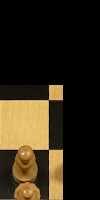
\includegraphics[width=1.9cm]{augmentation_orig}
    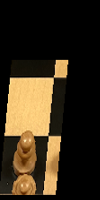
\includegraphics[width=1.9cm]{augmentation_0}
    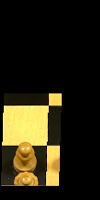
\includegraphics[width=1.9cm]{augmentation_1}
    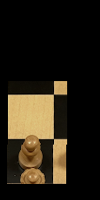
\includegraphics[width=1.9cm]{augmentation_2}
    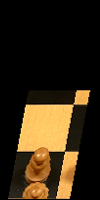
\includegraphics[width=1.9cm]{augmentation_3}
    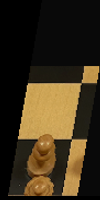
\includegraphics[width=1.9cm]{augmentation_4}
    \caption[The augmentation pipeline applied to an input image.]{The augmentation pipeline applied to an input image (left). Each output looks different due to the random parameter selection.}
    \label{fig:augmentations}
\end{figure}
The augmentation pipeline is applied to each image for each batch during training, meaning that different augmentations are used each time even though the underlying images might be the same.

\subsection{Fine-tuning}
\label{sec:transfer_learning_finetuning}
To train the networks, we follow a two-stage approach as motivated in \cref{sec:background_transfer_learning} and already employed in \cref{sec:occupancy_classification,sec:piece_classification}.
First, we train only the classification head with a learning rate of 0.001, and then we decrease the learning rate by a factor of ten and train all layers.
In the case of the occupancy classifier, we perform 100 iterations over the entire training set at both stages, essentially following the same regime as \cref{sec:occupancy_classification}.
However, for the piece classifier, we execute an additional 50 iterations in the second stage to ensure reliable convergence.
As expected, we are unable to achieve gains in the occupancy classifier's accuracy because it already achieved such a strong performance from the outset.
In fact, the loss is already below 0.001 at the beginning of training which can be seen in \cref{fig:transfer_learning_loss_accuracy_occupancy}.
\begin{figure}
    \centering
    \begin{subfigure}{\textwidth}
        \begin{tikzpicture}
            \begin{axis}[
                no markers,
                xlabel={step},
                ylabel={cross-entropy loss},
                title={Loss},
                scale only axis,
                width=.4\textwidth,
                legend style={at={(0.98,0.98)},anchor=north east}
            ]
                \addplot table [x=Step, y=Value, col sep=comma] {data/run-transfer_learning_occupancy_classifier_train-tag-Loss.csv};
                \addplot table [x=Step, y=Value, col sep=comma] {data/run-transfer_learning_occupancy_classifier_val-tag-Loss.csv};
                \legend{training,validation}
            \end{axis}
        \end{tikzpicture}
        \hfill
        \begin{tikzpicture}
            \begin{axis}[
                no markers,
                xlabel={step},
                ylabel={accuracy},
                title={Accuracy},
                scale only axis,
                width=.4\textwidth,
                ylabel near ticks,
                yticklabel pos=right,
                legend style={at={(0.98,0.02)},anchor=south east}
            ]
                \addplot table [x=Step, y=Value, col sep=comma] {data/run-transfer_learning_occupancy_classifier_train-tag-Accuracy.csv};
                \addplot table [x=Step, y=Value, col sep=comma] {data/run-transfer_learning_occupancy_classifier_val-tag-Accuracy.csv};
                \legend{training,validation}
            \end{axis}
        \end{tikzpicture}
        \caption{occupancy classifier}
        \label{fig:transfer_learning_loss_accuracy_occupancy}
    \end{subfigure}
    \par\vspace{1cm}
    \begin{subfigure}{\textwidth}
        \begin{tikzpicture}
            \begin{axis}[
                no markers,
                xlabel={step},
                ylabel={cross-entropy loss},
                title={Loss},
                scale only axis,
                width=.4\textwidth,
                legend style={at={(0.98,0.98)},anchor=north east}
            ]
                \addplot table [x=Step, y=Value, col sep=comma] {data/run-transfer_learning_piece_classifier_train-tag-Loss.csv};
                \addplot table [x=Step, y=Value, col sep=comma] {data/run-transfer_learning_piece_classifier_val-tag-Loss.csv};
                \legend{training,validation}
            \end{axis}
        \end{tikzpicture}
        \hfill
        \begin{tikzpicture}
            \begin{axis}[
                no markers,
                xlabel={step},
                ylabel={accuracy},
                title={Accuracy},
                scale only axis,
                width=.4\textwidth,
                ylabel near ticks,
                yticklabel pos=right,
                legend style={at={(0.98,0.02)},anchor=south east}
            ]
                \addplot table [x=Step, y=Value, col sep=comma] {data/run-transfer_learning_piece_classifier_train-tag-Accuracy.csv};
                \addplot table [x=Step, y=Value, col sep=comma] {data/run-transfer_learning_piece_classifier_val-tag-Accuracy.csv};
                \legend{training,validation}
            \end{axis}
        \end{tikzpicture}
        \caption{piece classifier}
        \label{fig:transfer_learning_loss_accuracy_pieces}
    \end{subfigure}
    \caption[Loss and accuracy in fine-tuning the occupancy and piece classifiers on the new dataset.]{Loss and accuracy in fine-tuning the occupancy and piece classifiers on the new dataset. Due to the limited availability of data, the validation set is simply the training set without augmentations. Both fine-tuned models achieve an accuracy of 100\% on the training data.}
    \label{fig:transfer_learning_loss_accuracy}
\end{figure}
Thus the ocupancy classifier achieves an accuracy of 100\% quite quickly during training, even before all layers are unfrozen halfway through the training.

On the other hand, the piece classifier starts with a loss value just under 2, and only converges during the second training stage which starts around step\footnote{Recall that the number of steps is different to the number of iterations over the dataset, due to the fact that the dataset consists of multiple batches.} 300, as depicted in \cref{fig:transfer_learning_loss_accuracy_pieces}.
Nonetheless, the convergence of the loss is relatively smooth.
The fluctuations in accuracy at the beginning of training can be explained by the small size of the dataset.

Key indicators for evaluating the performance of the chess recognition pipeline using the newly fine-tuned models on the transfer learning dataset are summarised in \cref{tbl:transfer_learning_results}.
\begin{table}
    \centering
    \begin{tabular}{lrr}
        \toprule
        metric & training set & test set \\
        \midrule
        mean number of incorrect squares per board           & 0.00     & 0.11 \\
        percentage of boards predicted with no mistakes      & 100.00\% & 88.89\%   \\
        percentage of boards predicted with $\leq 1$ mistake & 100.00\% & 100.00\%   \\
        per-board corner detection accuracy                  & 100.00\% & 100.00\% \\
        per-square occupancy classification accuracy         & 100.00\% & 99.88\% \\
        per-square piece classification accuracy             & 100.00\% & 99.94\% \\
        \bottomrule
    \end{tabular}
    \caption{Performance of the fine-tuned chess recognition pipeline on the transfer learning dataset.}
    \label{tbl:transfer_learning_results}
\end{table}
Comparing that to \cref{tbl:transfer_learning_results_without_finetuning}, we experience drastic improvements in all aspects.
Even in absolute terms, the results are very strong and a testament to the effectiveness of using transfer learning and careful data augmentation in order to adapt to a slightly different data distribution.
The mean number of incorrect squares per board decreased by almost two orders of magnitude to $0.11$.
This allowed an increase in the percentage of correctly identified positions from 0\% to 89\%. 
The remaining 11\% of positions were identified with just one mistake.
In other words, there were only three errors in all 27 samples in the test set.

\end{document}